\subsection{Reporting}

\subsubsection{scope}
\par{This section provides the details use case requirements for the use cases offered by the Authentication
module.}

\begin{figure}[h]
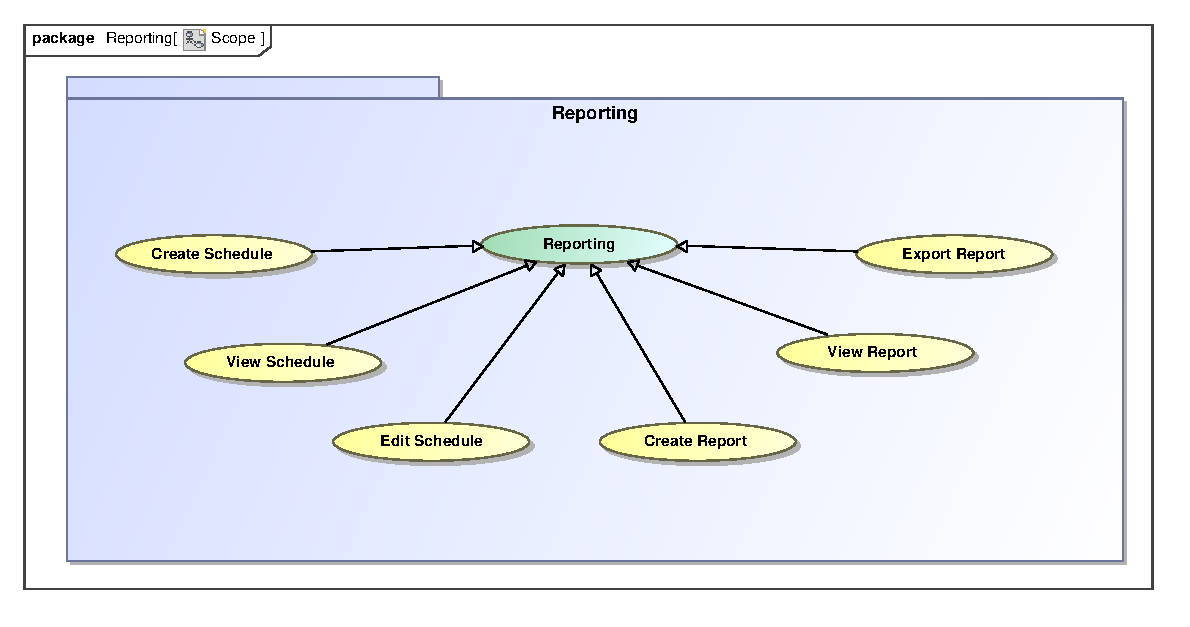
\includegraphics[height=250px, width=500px]{epsImages/Reporting/ReportScope.eps}
\caption{Scope of Reporting module}
\end{figure}


\subsubsection{Use Cases}

\begin{enumerate}
\item \textbf{CreateSchedule - priority: important}
\par{This use case allows a user to create a work schedule for the book that may consist of multiple tasks.}

\begin{figure}[h]
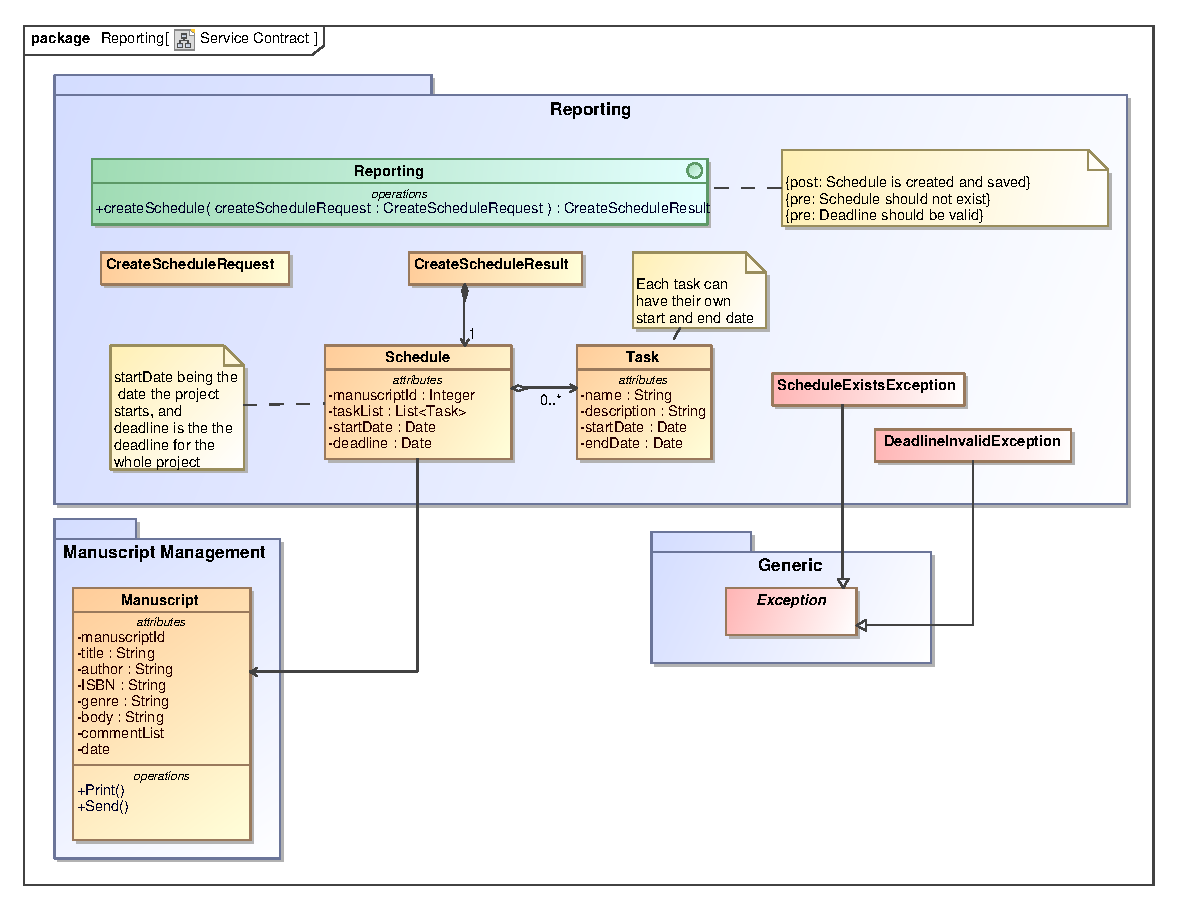
\includegraphics[height=250px, width=500px]{epsImages/Reporting/createSchedule.eps}
\caption{Service contract for creating a work schedule}
\end{figure}

\item \textbf{ViewSchedule - priority: important}
\par{This use case allows a user to view the work schedule for the book.}

\begin{figure}[h]
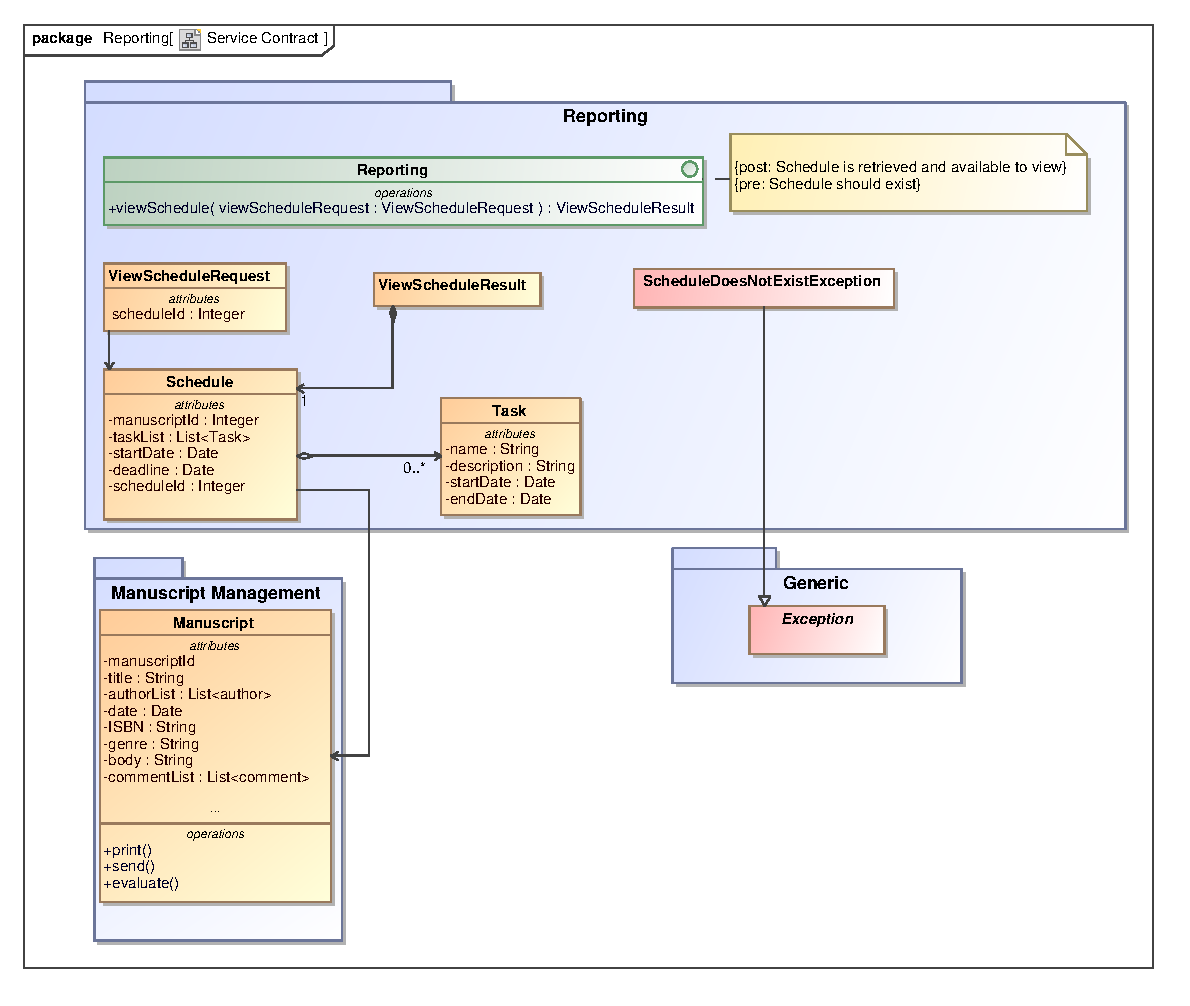
\includegraphics[height=250px, width=500px]{epsImages/Reporting/viewSchedule.eps}
\caption{Service contract for viewing a work schedule}
\end{figure}

\item \textbf{EditSchedule - priority: important}\\
\par{This use case allows a user to make changes to the work schedule of the book.}
\par{\textbf{service contract:} below is the service contract for editing a work schedule}

\begin{figure}[h]
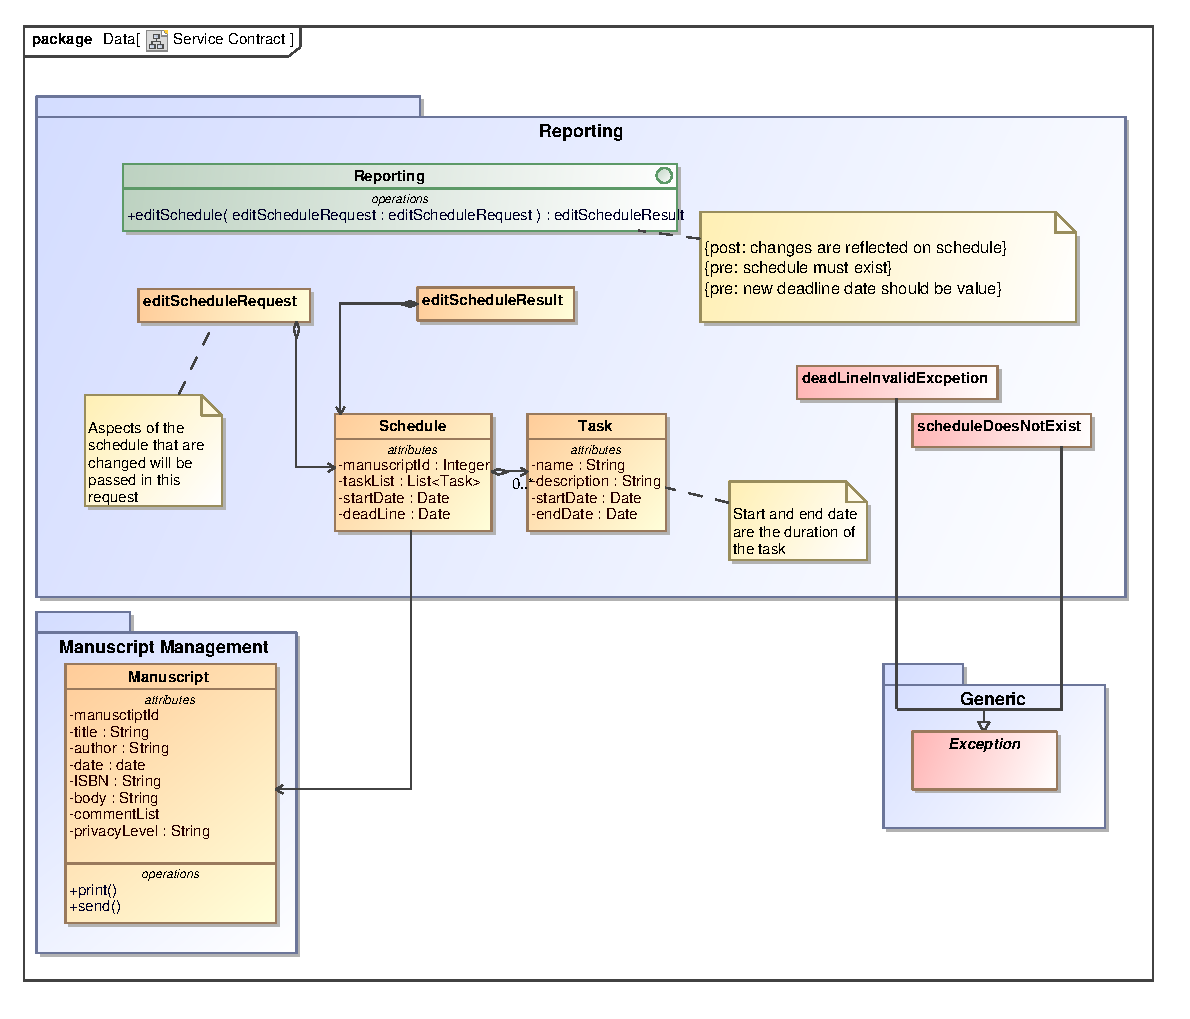
\includegraphics[height=250px, width=500px]{epsImages/Reporting/editScheduleServiceContract.eps}
\caption{Service contract for editing a work schedule}
\end{figure}

\item \textbf{createReport - priority: important}\\
\par{This use case creates  a report based on filters and provides it in printable format.}\\
\par{\textbf{service contract:} The service contract for the createReport  service is shown in figure below. The pre-conditions are enforced (raising the appropriate exception should they not be met) and the report is created and return in a printable format.}

\begin{figure}[h]
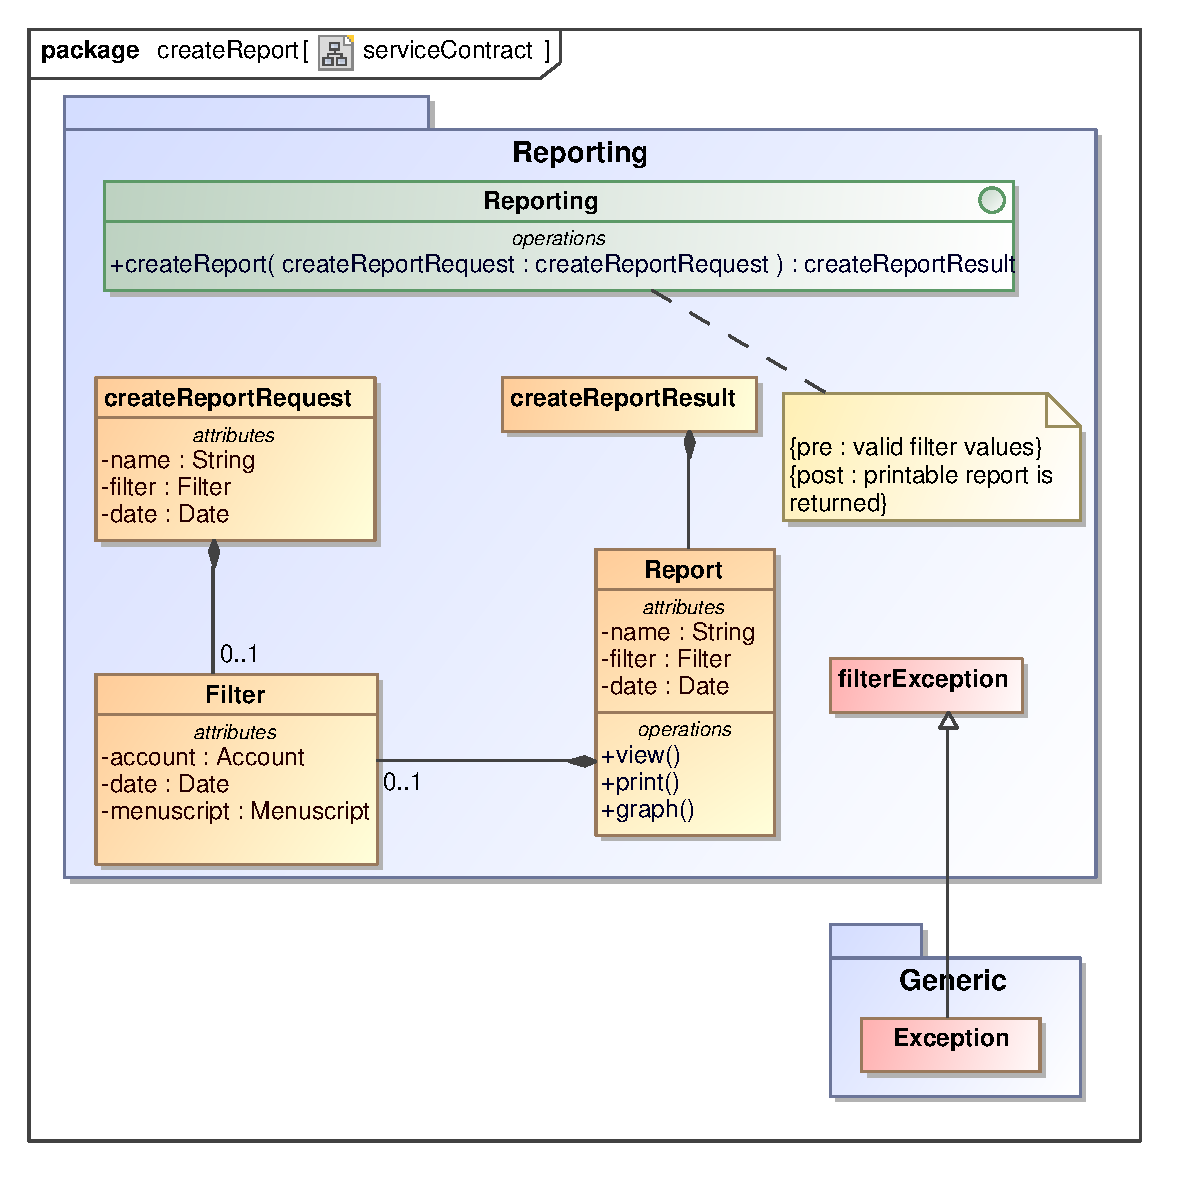
\includegraphics[height=250px, width=500px]{epsImages/Reporting/createReport.eps}
\caption{Service contract for creating a report}
\end{figure}

\item \textbf{viewReport - priority: important}\\
\par{This use case allows users to view a generated report, on the system (before exporting to say, a pdf for example).}\\
\par{\textbf{service contract:} Below is the service contract for viewing a report.}

\begin{figure}[h]
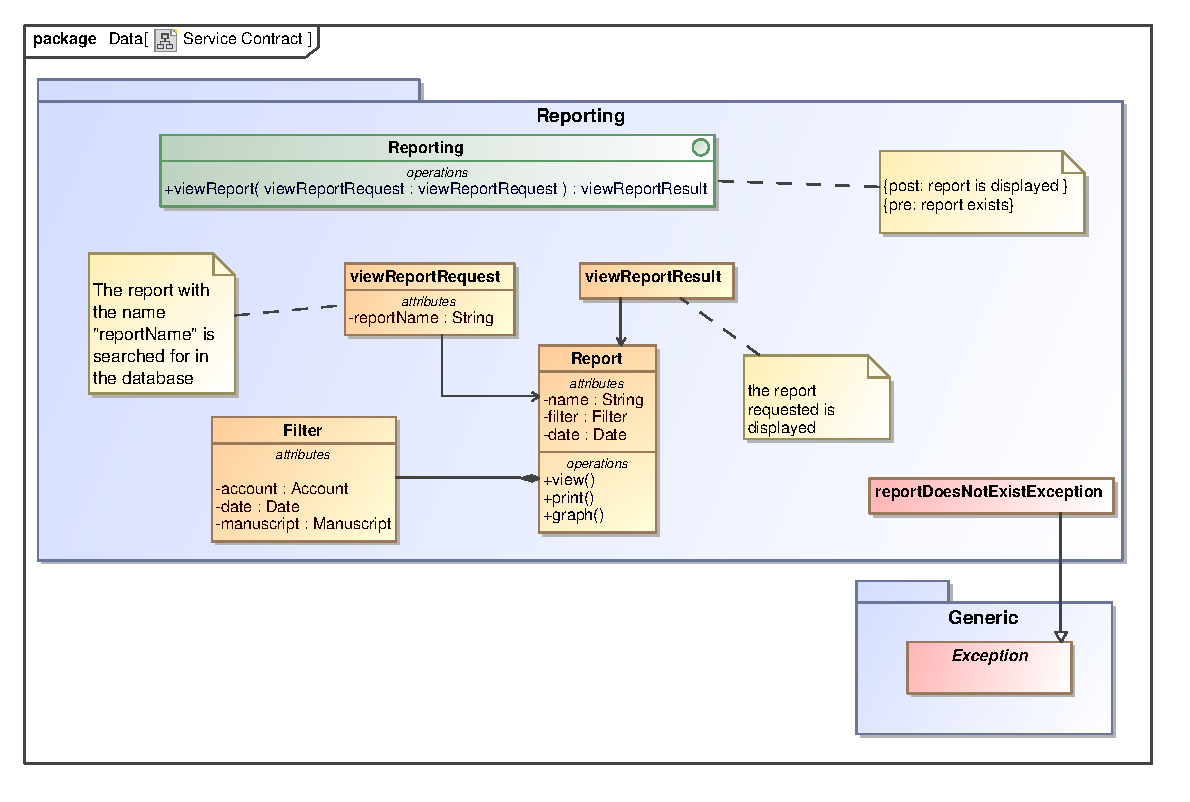
\includegraphics[height=250px, width=500px]{epsImages/Reporting/viewReportServiceContract.eps}
\caption{Service contract for viewing a report}
\end{figure}

 
\item \textbf{exportReport}
\par{priority: important  This use case which allows one to export a manuscript}\\
\par{\textbf{service contract:}} 

\begin{figure}[h]
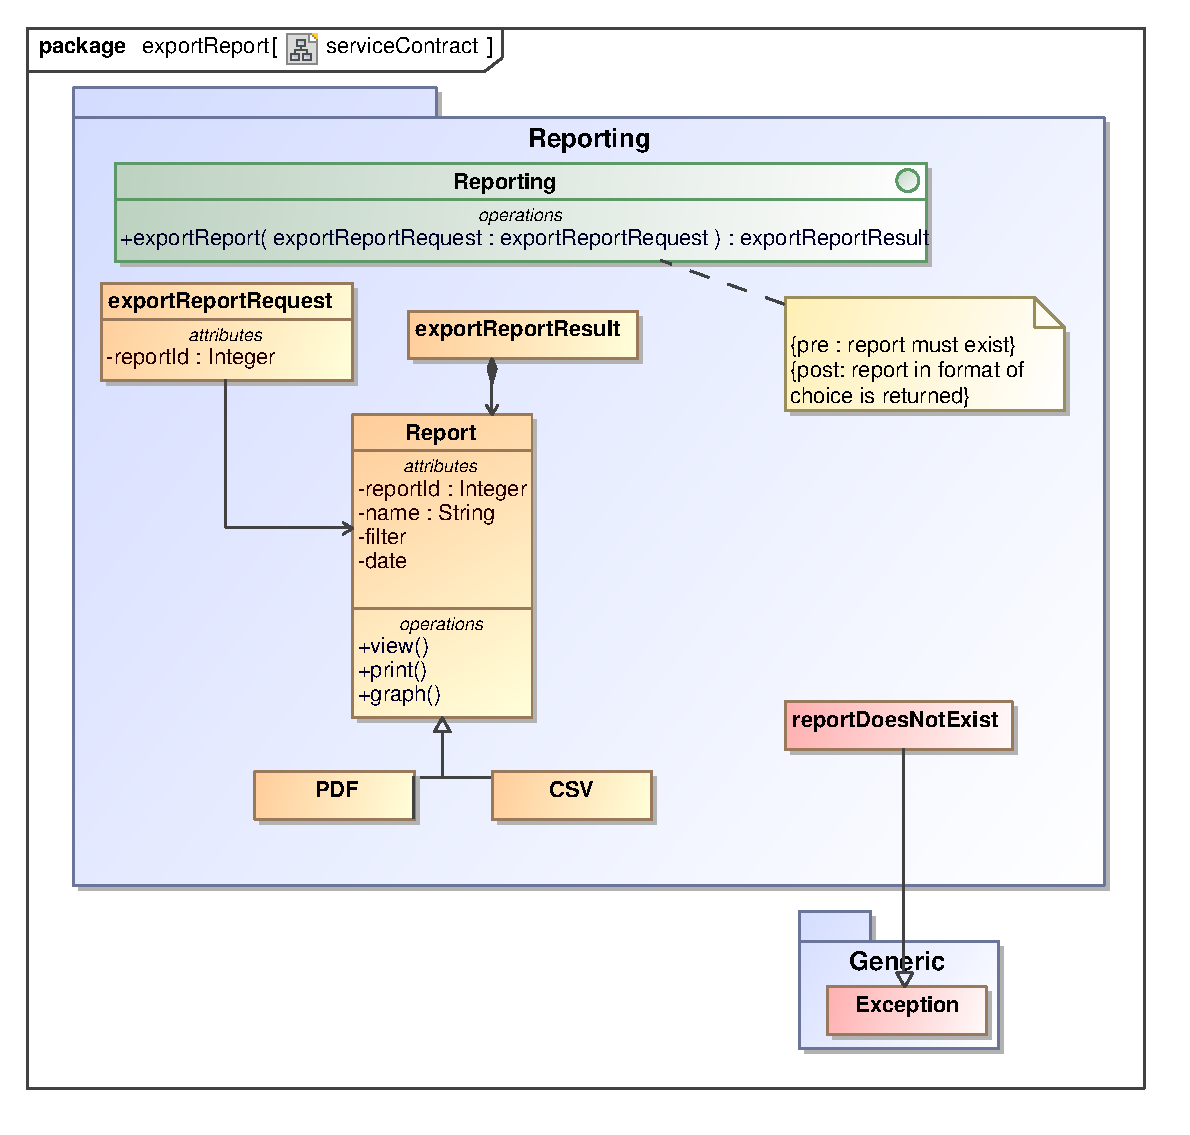
\includegraphics[height=250px, width=500px]{epsImages/Reporting/exportReport.eps}
\caption{Service contract for exporting a report}
\end{figure}
\end{enumerate}
